\documentclass[11pt]{article}

% \usepackage[margin=0.6in]{geometry}
\usepackage[T1]{fontenc}
\usepackage{array}
\usepackage{url}
\usepackage{graphicx}
\usepackage{background}
\usepackage{listings}

\backgroundsetup
{
	scale=1.0,
	angle=0,
	opacity = 1,
	contents = {%
		
\includegraphics[width=\paperwidth,height=\paperheight]{report/concordia-watermark.png}
	}%
}

\usepackage{xcolor}

\definecolor{codegreen}{rgb}{0,0.6,0}
\definecolor{codegray}{rgb}{0.5,0.5,0.5}
\definecolor{codepurple}{rgb}{0.58,0,0.82}
\definecolor{backcolour}{rgb}{0.95,0.95,0.92}

\lstdefinestyle{mystyle}{
    backgroundcolor=\color{backcolour},   
    commentstyle=\color{codegreen},
    keywordstyle=\color{magenta},
    numberstyle=\tiny\color{codegray},
    stringstyle=\color{codepurple},
    basicstyle=\ttfamily\footnotesize,
    breakatwhitespace=false,         
    breaklines=true,                 
    captionpos=b,                    
    keepspaces=true,                 
    numbers=left,                    
    numbersep=5pt,                  
    showspaces=false,                
    showstringspaces=false,
    showtabs=false,                  
    tabsize=2
}

\lstset{style=mystyle}


\title{Cm VM Port for the\\ATmega328P Microcontroller}

\author{
\begin{tabular}{c}

\begin{tabular}{r l}
    Nataliya Dimitrova & 24662407 \\
    Matthew Massey & 40061791 \\
    Jon Zlotnik & 40030143
\end{tabular}\\ \\
Team \#10 \\ 
(Burnt Socket)\\ \\ \\
\\ \\ \\ \\ \\
Project Report for SOEN 422\\ \\
\url{https://github.com/M-Massey/cmvm-atmega328p}\\
\\ \\ \\
Engineering and Computer Science\\
Concordia University\\
Montreal, QC, Canada
\end{tabular}
}

\date{December 7, 2020}

\begin{document}

\maketitle
\thispagestyle{empty}

\clearpage
\pagenumbering{arabic} 

\tableofcontents

\vspace{10mm}

N.B. Our implementation can run all 12 tests from the ``big'' test suite as well as the newer small tests.

\newpage

\section{Introduction}

% This section provides a short description of your project. Discuss what hardware and software were used.

Our port of the Cminor (Cm) virtual machine (VM) is written in ANSI C for the Aruino Nano, equipped with the ATmega328P 8-bit microcontroller (MCU).
This ported virtual machine can be compiled using Microchip's AVR-GCC cross-compiler.
Specifically, we depend on the I/O (i.e. \lstinline[columns=fixed]{<avr/io.h>}) and interrupt (i.e. \lstinline[columns=fixed]{<avr/interrupt.h>}) libraries that come with the AVR toolchain.

The workstations used to develop the port were running Windows 10, but the AVR toolchain, our build and test scripts written in PowerShell Core, and the Cm program loader written in dotNet core are all cross platform.
So you shouldn't have any barriers preventing you from building the project from source.


\section{Goal of the Project}

% This section provides a quick overall summary of what your group’s tasks have achieved during the port of the virtual machine on the Arduino Nano.

The project required three major development efforts. The first was porting functionality from a DOS/Win32 architecture to an 8-bit architecture. 
All code that depended on platform specific libraries was abstracted away by a board specific layer (BSL). 
We then implemented the same functionality in an ATmega328P BSL and added interrupt management as well as the ability to read and write to the MCU's I/O registers by address.
Finally, preprocessor directives were added in the hardware abstraction layer (HAL) so that the appropriate BSL could be selected at compile-time.

The second dev effort was extending the Cm program loader.
This consisted of adding to the provided serial loader, written in C\#, to accommodate larger files of Cm bytecode and verifying the integrity of the packets sent over UART to the Arduino Nano.
An additional ``admin'' driver for the VM running on the MCU needed to be written to allow for bytecode loading, execution, and verification over UART.

Lastly, build and deployment scripts were written to ensure consistent testing of the project across workstations. 
Admin drivers for functionality tests agnostic of the serial loader were also included in the VM source.





\section{Implementation of Tasks}
% This section should summarize your implementation of the following main tasks on the target:

% Theses subsections are expected to have the discussion of the implementations as well. You should include snippets of code that your group feels are relevant (and proud) to your project’s overall functionality. Do not simply toss in code but rather, discuss what is relevant about the code of the specific task and where it belongs. Theses subsections serve also as a reflection of the tasks. Discuss which tasks were met, which weren’t and why.

\subsection{Task 3: BSL and HAL layers}

The BSL layer was carved out of the original VM source by identifying potentially platform-specific implementations and giving them generic interfaces. With the DOS/Win32 layer abstracted away, we duplicated each interface and implemented them, this time, with code that depended on AVR libraries instead of DOS libraries. 

For example, \lstinline[columns=fixed]{_avr_cout.c} to exposes the same factory but uses the \lstinline[columns=fixed]{USART_Transmit(unsigned char data)} function from \lstinline[columns=fixed]{_avr_uart.h} to perform the actual character ``putting'' instead of \lstinline[columns=fixed]{printf()} or \lstinline[columns=fixed]{putchar()} as seen in the DOS BSL.

\begin{center}
    \begin{lstlisting}[language=C, columns=fixed, caption=Beginning of \_avr\_cout.c]
#include "_avr_outdesc.h"
#include "_avr_xtoa.h"
#include "_avr_uart.h"

#define FOSC  16000000 // Clock Speed
#define BAUD 57600
#define MYUBRR FOSC/16/BAUD-1

static void TxChar(char c) { USART_Transmit(c); }

static void Console_Putchar(char c) { TxChar(c); }

...
    \end{lstlisting}
\end{center}


To further illustrate the concept, in task 6, we wrote \lstinline[columns=fixed]{_win_interrupts.h} and \lstinline[columns=fixed]{_avr_interrupts.h} such that both effectively expose the same generic interface:

\begin{center}
    \begin{lstlisting}[language=C, columns=fixed, caption=Generic interface example.]
void __cli();
void __sei();

u16 __saveAndDisable();
void __restore(u16 flags);
    \end{lstlisting}
\end{center}

The DOS implementation depends on the windows specific \lstinline[columns=fixed]{<dos.h>} header and i386/amd64 op codes.
The AVR implementation, on the other hand, is dependent on Microchips's AVR libraries as can be seen below in \lstinline[columns=fixed]{_avr_interrupts.c}:

\begin{center}
    \begin{lstlisting}[language=C, columns=fixed, caption=\_avr\_interrupts.c]
#include "_avr_interrupts.h"

#include <avr/io.h>
#include <avr/interrupt.h>

void  __cli(void) { cli(); }
void  __sei(void)  { sei(); }

u16   __saveAndDisable(void) { 
    u16 flags =  SREG;
    __cli();
    return flags;
}

void  __restore(u16 flags) {
    SREG = flags;
}
    \end{lstlisting}
\end{center}

We chose to add the \lstinline[columns=fixed]{_[arch]_} prefix to denote files that have a high probability of needing to be re-implemented upon platform change. They compose our BSL.

Files without a prefix are either part of the hardware abstraction layers or are admin drivers which orchestrate the HAL and sometimes the BSL.

The HAL code is responsible for providing platform agnostic interfaces and implementation that can execute Cm bytecode. Such platform agnostic code can be seen in \lstinline[columns=fixed]{interman.c} and \lstinline[columns=fixed]{interman.h}.

\begin{center}
    \begin{lstlisting}[language=C, columns=fixed, caption=interman.c]
#include "interman.h"

void  Interrupt_Disable(void) { __cli(); }
void  Interrupt_Enable(void)  { __sei(); }

u16   Interrupt_SaveAndDisable(void) { 
    return __saveAndDisable(); 
}
void  Interrupt_Restore(u16 flags) { 
    return __restore(flags);
}
    \end{lstlisting}
\end{center}

\begin{center}
    \begin{lstlisting}[language=C, columns=fixed, caption=interman.h]
#ifndef __interman_h
#define __interman_h

#ifdef AVR
#include "_avr_stdtype.h"
#include "_avr_interrupts.h"
#else
#include "_win_stdtype.h"
#include "_win_interrupts.h"
#endif

void  Interrupt_Disable(void);
void  Interrupt_Enable(void);
u16   Interrupt_SaveAndDisable(void);
void  Interrupt_Restore(u16 flags);

#endif
    \end{lstlisting}
\end{center}

As you can see above, in Listing 4, we allow for platform choice at compile time with command line ``define'' arguments (e.g. \lstinline[columns=fixed]{avr-gcc -DAVR [...]}).


\subsection{Task 4: VM Operand Stack and the VM core}

Running the pre-compiled tests, at this point, was simply a matter of calling the HAL implementation from hard-coded "admin" drivers such as the following:

\begin{center}
    \begin{lstlisting}[language=C, columns=fixed, caption=admin\_avr\_test\_t11.c]
#include "hal.h"
#include "out.h"
#include "vm.h"

u8 data[] = { 0xE1, 0x00, 0x25, 0x71, 0xD5, 0x00, 0x2F, 0xFF, 0x85, 0xD5, 0x00, 0x44, 0xFF, 0x85,
0xD9, 0x09, 0xA8, 0xE0, 0x0E, 0xA0, 0x90, 0x1C, 0xE3, 0x04, 0xE0, 0x09, 0xA0, 0xB4, 0x00, 0xFF,
0x82, 0xE0, 0xF4, 0xFF, 0x87, 0x03, 0x04, 0xE7, 0xFF, 0xFF, 0xE7, 0xFF, 0xDB, 0x00, 0x54, 0x2E,
0x53, 0x74, 0x6D, 0x74, 0x00, 0x54, 0x65, 0x73, 0x74, 0x20, 0x31, 0x31, 0x3A, 0x20, 0x62, 0x72,
0x65, 0x61, 0x6B, 0x20, 0x53, 0x74, 0x61, 0x74, 0x65, 0x6D, 0x65, 0x6E, 0x74, 0x0A, 0x00, 0x39,
0x38, 0x37, 0x36, 0x35, 0x34, 0x33, 0x32, 0x31, 0x30, 0x0A, 0x00  };
/*public*/  u8*    mem = data;

int main (void) {
    
    Hal_Init();
    VM_Init(mem);
    VM_execute(mem);
}
    \end{lstlisting}
\end{center}

As you can see, we simply passed the Cm bytecode to the VM without reference to AVR or DOS headers.

\subsection{Task 5: Serial Loader on the target}

Serial loading of the Cm bytecode required both a workstation client and a VM admin driver.
The workstation client compiles to an executable \lstinline[columns=fixed]{cmload} which takes two arguments: the bytecode file, and the target port. 
There are issues with multi-packet data transmission due to unstable multithreaded sharing of the serial port.
When analyzing the running executable in procmon, from Windows Sysinternals, you can see it spin up a whole bunch of threads that end up interfering with each other's operation.
Fortunately, the bytecode almost always gets transmitted properly, and the serial output of the VM is usually visible in the output of the \lstinline[columns=fixed]{cmload} command-line app.

The steps we took towards development of the workstation client were divided into three milestones.
The first was to achieve single packet transmission which would provide just enough bytecode to print a single character.
\begin{figure}[h!]
    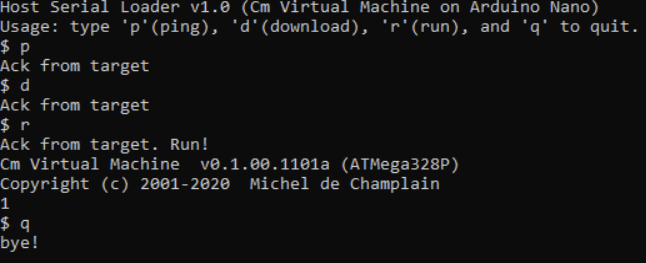
\includegraphics[width=\textwidth]{report/single_predefined_packet.PNG}
    \caption{Single packet serial transmission}
\end{figure}

The second was to be able to verify the integrity of the individual packets.
We achieved this through the passing of Acks and Nacks and checking them after every transmission.
A simple checksum was used on the MCU and on the workstation to summarize and verify integrity of packets.
You can see example output from the workstation client in the following figures.

\begin{figure}[h!]
    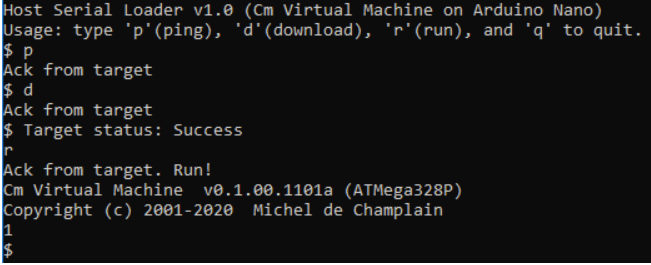
\includegraphics[width=\textwidth]{report/checksum_valid.PNG}
    \caption{Successful transmission with only Acks}
\end{figure}

\begin{figure}[h!]
    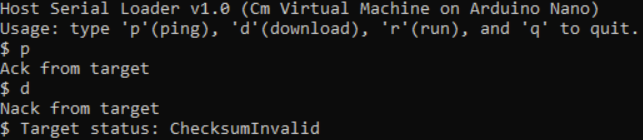
\includegraphics[width=\textwidth]{report/checksum_invalid.PNG}
    \caption{Unsuccessful transmission with Nacks}
\end{figure}

The last milestone was to achieve a successful multi-packet transmission. We did this by modifying the workstation client to read a file, split it up into packets with appropriate headers, and finally send them. Each packet has a maximum size of 11 useful bytes: 3 bytes for the header, and 8 bytes of data.

\begin{figure}[h!]
    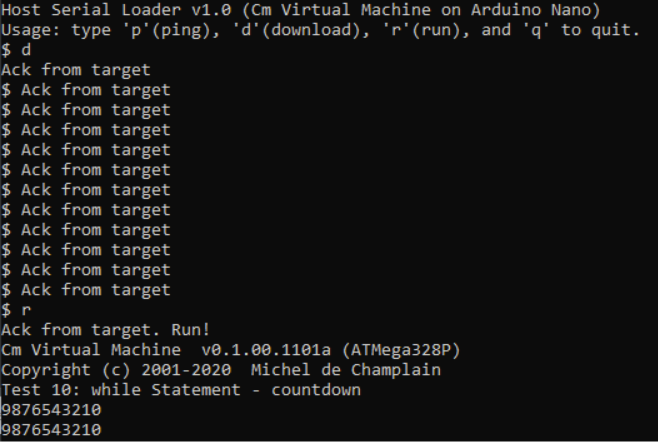
\includegraphics[width=\textwidth]{report/multipacket_run.PNG}
    \caption{Successful download and execution of multipacket bytecode file, namely Test 10 from the test suite.}
\end{figure}

The admin driver we implemented for the target MCU (i.e. \lstinline[columns=fixed]{admin_avr_serial_loadable.c}) was responsible for sending Ack, Nacks, and status packets in addition to regular VM console output.
It loops while receiving packets from the host and computes the checksum of every packet.
The contents main loop are detailed in Listing 7.

\begin{center}
    \begin{lstlisting}[language=C, columns=fixed, caption=Main loop body of admin\_avr\_serial\_loadable.c]
u8 len = USART_Receive(); //receive lenght of incoming packet
if (len < 3){   // the min lenght of a packet is 3 bytes
    status = InvalidAddr;
    continue;
}else {
    mem = uart_get(len-1); // receive the packet without the size byte because we already got it
    u8 zero = USART_Receive(); // receive zero   

    verifyChecksum = checksum(len-1, mem);
    chunkSize = len-3;  // payload in packet
}

switch(mem[1]){  // mem[1] is the commnad 
    case 32: {   // ping
        sendAck();
        status = SuccessCmd;
    } break;
    case 36: { // receiving data
        if(chunkSize) {

            if(verifyChecksum == 1){
                ptr = (u8*)realloc(ptr,dataSize+chunkSize);
                memcpy(ptr + dataSize, mem+2, chunkSize);
                dataSize += chunkSize;
                status = SuccessCmd;
                sendAck();
            }else {
                status = ChecksumInvalid;
                sendNack();
            }   
        }
        else{
            status = InvalidAddr;
            sendNack();
        }
       
    } break;
    case 34: {  // run
        sendAck();
        DisplayBanner();
        VM_Init(ptr);
        VM_execute(ptr);
        sendAck();
        status = SuccessCmd;
        free(ptr);
        ptr = 0;
        resetFunc();
        
    } break;
    case 35: {  // getStatus
        //sendAck();
        sendStatus(status);
    } break;
    default: {
        status = UnknownCmd;
    }
}
free(mem);
USART_Flush();
    \end{lstlisting}
\end{center}




\subsection{Task 6: Interrupt functions}

\begin{figure}[h!]
    \centering
    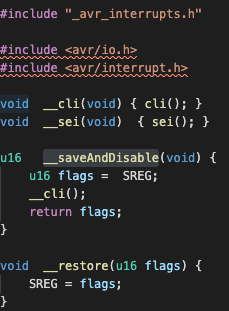
\includegraphics[height=3in]{report/Interman_Implementation.png}
    \caption{\_\_avr/io.h Implementation.}
\end{figure}
Implementation of the interrupts were handled within \lstinline[columns=fixed]{_avr_interrupts.c}. (See Figure 5)
We added imports of 'avr/io.h' and 'avr/interrupt.h' to have access the avr methods. \_\_cli(void) and \_\_sei(void) functions are set to their avr equivalents of cli() and sei() to disable and enable interrupts. For the implementation of \_\_saveAndDisable we store the current value of SREG (Status Register), we then disable interrupts and return the value of the stored SREG. For \_\_restore(u16 flags) we simply set the value of SREG to the value of the passed 'flags' parameter. At first we thought of using EIFR (External Interrupt flag register), but after testing with SREG and matching the tests we concluded it made sense to store SREG before and interrupt would take place. (See Figure 6.)

\begin{figure}[h!]
    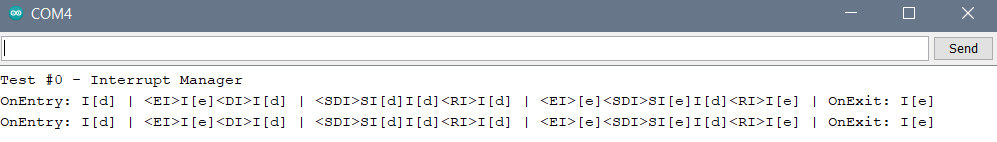
\includegraphics[width=\textwidth]{report/working_interman_test.PNG}
    \caption{Successful execution of hard coded (not serial loaded) interrupt manager test.}
\end{figure}

\subsection{Task 7: I/O Register functions}

The IO register functions were relatively simple to write as demonstrated in listing 8. 
We simply used the same macro the AVR library uses to transform the register name macros like \lstinline[columns=fixed]{DDRB} or \lstinline[columns=fixed]{PORTB} into their mapped address.
Also note, interrupts are disabled and restored/re-enabled during register operations so as not to have indeterministic values in the registers.

\begin{center}
    \begin{lstlisting}[language=C, columns=fixed, caption=Register manipulation implementation from \_avr\_ioreg.c.]
// Software internal counters and values
static u32 _nReads;
static u32 _nWrites;

u32 bsl_IOReg_Read(u32 port) {
    u16 temp_flags = __saveAndDisable();
    ++_nReads;
    u32 out = _SFR_IO8((u8)port);
    __restore(temp_flags);
    __sei();
    return out;
} 

void bsl_IOReg_Write(u32 port, u32 value) {
    u16 temp_flags = __saveAndDisable();
    ++_nWrites;
    _SFR_IO8((u8)port) = (u8)value;
    __restore(temp_flags);
    __sei();
}
    \end{lstlisting}
\end{center}


\section{Conclusion}
Most initial issues faced were due to differring development environments among team members. Later, typos/inconsistencies in the provided source code were the main hurdles. We managed to work around the differring development environments by compiling the serial loader's workstation client in dotNet core and writing build/upload scripts in PowerShell Core. As long as we didn't depend on Windows specific extensions to the .net framework, the code would be cross platform. Understanding the provided code samples and trying to re-implement the DOS specific op code to be ATmega328P compatible proved chanllenging, but after reading through the i386 and AMD64 op tables, we began to understand what we needed to accomplish as a group. If we were more experienced with assembly, the initial comprehension hurdles would have probably been overcome more quickly. Once we made sense of it all some tasks took barely any effort when using the avr libraries. 
\end{document}

% meh...
% aight, let's call it?